\subsection{Black hole radiation according to Hawking N} 
	We now have a closer look to a one-sided black hole which was created by a collapse. As discribed in the caption of \textbf{Figure \ref{collapse}}, just the section above the shell is Schwarzschild geometry, below we have Minkowski geometry. This means, that the solutions we found in the section before are just usefull for above the shell. The solutions below the shell come from the Minkowski wave equation and are plaine wave kind. These the first must get matched with the second, otherwise we won't have a solution for the hole space-time.
	
	The difficulty is, that there even is no global time-translation symmetry. 
	\begin{figure}
		\begin{center}
			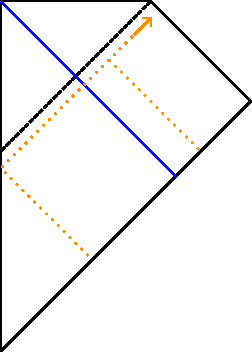
\includegraphics[scale=1]{collapse2}
			\caption{This is the geometry for a black hole made from collapse. Other than in \textbf{Figure \ref{collapse}} the collapsing shell is here shown in blue.} \label{collapse2}
		\end{center}
	\end{figure}